\documentclass[addpoints,11pt,a4paper]{exam}
\printanswers
\usepackage{amsmath, amssymb, amsthm}
\renewcommand{\rmdefault}{ppl} % rm
\linespread{1.05}        % Palatino needs more leading
\usepackage[scaled]{helvet} % ss
\usepackage{courier} % tt
\usepackage{eulervm} % a better implementation of the euler package (not in gwTeX)
\normalfont
\usepackage{caption}
\usepackage[T1]{fontenc}
\usepackage{mathrsfs}
\usepackage{tikz}
\usetikzlibrary{arrows, decorations.markings}
\usepackage{comment}
\usepackage{graphicx}
\usepackage[ruled,vlined,linesnumbered, resetcount]{algorithm2e}
\usepackage{chemformula}
\usepackage{ulem}
\usepackage{paralist}
\usepackage{psfrag}
\usepackage{fullpage}
\usepackage{fancybox}
\usepackage{ifthen}
\usepackage{hyperref}
\hypersetup{
    colorlinks=true,
    linkcolor=blue,
    filecolor=magenta,      
    urlcolor=blue,
}
\usepackage{marvosym}
%%%%%%%%%%%%%%%%%%%%Code%%%%%%%%%%%%%%%%%%%%%%%%%%
\usepackage{listings}
\usepackage{color}
 
\definecolor{codegreen}{rgb}{0,0.6,0}
\definecolor{codegray}{rgb}{0.5,0.5,0.5}
\definecolor{codepurple}{rgb}{0.58,0,0.82}
\definecolor{backcolour}{rgb}{0.95,0.95,0.92}
 
\lstdefinestyle{mystyle}{
    backgroundcolor=\color{backcolour},   
    commentstyle=\color{codegreen},
    keywordstyle=\color{magenta},
    numberstyle=\tiny\color{codegray},
    stringstyle=\color{codepurple},
    basicstyle=\footnotesize,
    breakatwhitespace=false,         
    breaklines=true,                 
    captionpos=b,                    
    keepspaces=true,                 
    numbers=left,                    
    numbersep=5pt,                  
    showspaces=false,                
    showstringspaces=false,
    showtabs=false,                  
    tabsize=2
}

%%%%%%%%%%%%%%%%%%%%%%%%%%%%%%%%%%%%%%%%%%%%%
\usepackage[export]{adjustbox}
\extrawidth{1in}
\usepackage{multicol}
\setlength{\columnsep}{.001cm}
\newcommand{\twopartdef}[4]
{
	\left\{
		\begin{array}{ll}
			#1 & \mbox{if } #2 \\
			#3 & \mbox{if } #4
		\end{array}
	\right.
}
\newcommand{\G}{\mathcal{G}}
\newcommand{\fH}{\mathcal{H}}
\newcommand{\M}{\mathcal{M}}
\title{CS6730 : Assignment 1}
\author{Instructor and TAs}
\date{Release: 26th Feb 2019; {\bf Due: Mar 7th, 11.59pm}}

\begin{document}
\maketitle
\noindent\rule{\textwidth}{1pt}
\begin{itemize}
    \item Submit to {\bf GradeScope a single LaTeX-generated pdf file} containing your solutions. Please type your answers in the solutions blocks in the source LaTeX file of this assignment. 
    \item The final question worth half overall points is a programming assignment that asks for (a) the formulas you used, (b) a well-documented code you wrote, and (c) submission of predictions from your code to a kaggle competition. 
    \item You are encouraged to collaborate/discuss with other students on this assignment, but write your solutions/code in your own words.
\end{itemize}
\noindent\rule{\textwidth}{1pt}

\begin{questions}
\question[6]{\sc [How tree-like are you?]} 
Let $H$ be an undirected graph with $n$ nodes. Let $T(H)$ be the set of all chordal graphs with $n$-nodes that contain all edges in $H$. The tree width of $H$ is defined as $\text{min} \{ \text{Max-Clique}(H')-1:H'\in T(H)\}$. 
\begin{parts}
\part[4] What is the tree-width of the $n\times n$ grid graph containing $n^2$ nodes?  Give proof.  (Hint: Answer scales linearly with $n$.)
\begin{solution}
Given a graph $G$, we can add edges to it to make it chordal by considering an elimination ordering and at each step $i$ choosing $i$th vertex in ordering, remove it and adding extra edges between in its neighbors if not present(this ordering is the perfect elimination ordering of resultant chordal graph).


Any graph $H'$ in $T(H)$ can be constructed by first adding extra edges via an elimination ordering and then adding extra edges, which would only increase the value of $ \text{Max-Clique}(H')$.


Then, the tree-width is the largest subset of nodes in a note of clique-tree of $H'$ minus one. Because Clique-Tree nodes captures all maximal cliques of $H'$.


Let a $n\times n$ grid graph have vertices  $V=[n]\times [n]$($[n]=\{1,2,\dots,n\}$) and edge set $(i,j),(k,l)\in E$ iff $|i-j|+|k-l|=1$. Let $S=((1,1),(1,2),\dots,(1,n),(2,1)\dots,(2,n)\dots, (n,1)\dots,(n,n))$ be a sequence. First we add edges to make sub-graph induced by $((1,1),(1,2),\dots,(1,n),(2,1))$ a clique, then we add edges to make subgraph induced by $((1,2),(1,3),\dots,(1,n),(2,1),(2,2))$ be clique. We continue till subgraph induced by $((n-1,n),(n,1),(n,1)\dots,(n,n))$ is a clique. The resultant graph $H'$ is chordal since ordering of $S'=((n,n),(n,n-1),\dots,(n,1),(n-1,n)\dots,(n-1,1)\dots, (1,n)\dots,(1,1))$ is a perfect elimination ordering of $H'$ since for each vertex all their neighbors are either eliminated or occur in one of the cliques we have induced by adding edges in above process.For a node $(i,j)$ the neighbor farthest to right in $S'$ is $(i-1,j)$ and vertices $\{(i,j-1)\dots,(i,1),(i-1,n)\dots,(i-1,j-1)\}$ induce a clique by above process of edge addition.


Also the maximal clique is of size $n+1$, taking any one of above induced cliques and noting that for any two cliques $C_i,C_j$ which are created one after other the two vertices in $V(C_i)\bigoplus V(C_j)$ are not connected(they are of form $(i,j),(i+1,j+1)$ or $(i,n),(i-2,1)$), and hence tree-width of grid graph is atmost $n$.


To prove that tree-width is exactly $n$ is more involved(Refer Diestel- Graph Theory Chapter 12). We define following terms.\\
\textbf{Bramble:} a bramble for an undirected graph $G$ is a family of connected subgraphs of $G$ such that for any two disjoint subgraphs there exist an edge with one vertex in each of the two subgraphs.

\textbf{Order of Bramble:} It is the size of smallest set(hitting set) whose intersection with any of the vertex set of subgraphs is non-empty.

\textbf{Seymour , Thomas Theorem} A graph has tree-width $\geq k$ iff these exists a bramble of order $>k$.


\textbf{Claim:} A $n\times n$ grid graph has a bramble of order $n+1$.
\begin{proof} 

For a $k\times k$ subgraph we can get a bramble of order $k$ by considering family of subgraphs $\{G(i,j)|1\leq i,j \leq n,\}$ where $G(i,j)$ is the graph induced by vertices $\{(x,y)|x=i \text{or} y=j\}$. Graphs $G(i,j),G(m,l)$ have common vertices $\{(i,l),(m,j)\}$. The hitting set is vertices of any one of the diagonals: $\{(i,i)|i\in [k]\}$. Thus this bramble has order $k$.

For a grid graph $(k+1)\times (k+1)$, we need to construct a bramble of order atleast $k+2$. Consider the forst $k$ rows and columns. We start off with the abouve bramble for $k\times k$ subgraph. We then add two more subgraphs: One induced by all vertices in $\{(i,k+1)|i\in [k+1]\}$ and other $\{(k+1,i)|i\in [k]\}$. It is easy to see that addition of these two subgraphs forms bramble on $(k+1)\times (k+1)$ graph with smallest hitting set being all $k$ nodes on diagonal:$\{(i,i)|i\in [k+1]\}$ and any one node from last row say $(k+1,k)$(Since $(k+1,k+1)$ is not in the last subgraph). So the order is $k+2$.

\end{proof}

\textbf{Note:} The idea of proof sketch is from Diestel- Graph Theory Chapter 12. The above proof for claim is original contribution.

\end{solution}
\part[2] What is the tree width of the cycle graph with $n$ nodes? Give proof. (Hint: Answer does not depend on $n$.)
\begin{solution}
Any cycle has tree-width 2.\\
Let $C$ be a cycle $(v_1,v_2,\dots,v_n)$. If $n=3$, it is chordal and has tree-width 2.
Consider any elimination order on $C$ in order of cycle $(v_1,v_2,\dots,v_n)$, at every step $i$, the 2 neighbors of selected vertex is connected to get a new cycle $(v_{i+1},v_{i+2}\dots, v_n)$.(no other edges are added)\\
The Clique tree generated has nodes containing vertices of form $\{v_{i},v_{i+1},v{i+2}\}\forall i\in \{1,\dots,n-2\}$ along with $\{v_{n-1},v_{n},v{1}\}$, $\{v_{n},v_{1},v{2}\}$. Thus tree-width is atmost $3-1=2$ and since any chordal graph has a clique of size 3, tree-width is exactly 2.

\end{solution}
\end{parts}

\question[7]{\sc [Naive gets disoriented]}
\begin{parts}
\part[1] Give the MN structure and distribution for the Naive Bayes model, with the class label \textit{Y} taking values in the set $\{1,2, \ldots,n\}$ and feature values $X_1,\ldots,X_n$ taking values in $\{0,1\}$.
\begin{solution}
The BN structure that is a perfect I-map for Naive Bayes model is:\\
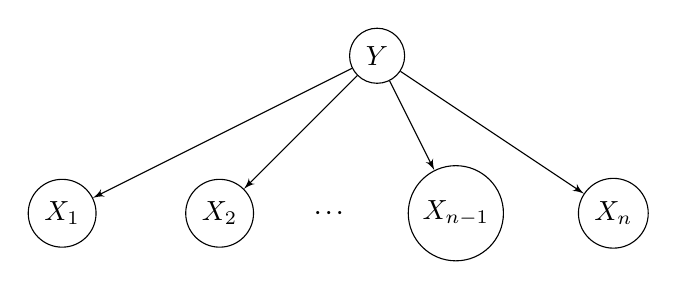
\begin{tikzpicture}
\tikzset{vertex/.style = {shape=circle,draw,minimum size=1.5em}}
\tikzset{edge/.style = {->,> = latex'}}
% vertices
\node[vertex] (Y) at  (4,2) {$Y$};
\node[vertex] (X1) at (0,0) {$X_1$};
\node[vertex] (X2) at (2,0) {$X_2$};
\node[vertex] (X3) at (5,0) {$X_{n-1}$};
\node[vertex] (X4) at (7,0) {$X_{n}$};

\draw [edge] (Y) to (X1);
\draw [edge] (Y) to (X2);
\draw [edge] (Y) to (X3);
\draw [edge] (Y) to (X4);

\path (X2) to node {\dots} (X3);

\end{tikzpicture}
with independencies $(X_i\perp X_j|Y) \forall i\neq j$.\\
This BN has no immoralities and is chordal thus the equivalent MN is:\\
\begin{tikzpicture}
\tikzset{vertex/.style = {shape=circle,draw,minimum size=1.5em}}
\tikzset{edge/.style = {-,> = latex',arrowhead=1cm}}
% vertices
\node[vertex] (Y) at  (4,2) {$Y$};
\node[vertex] (X1) at (0,0) {$X_1$};
\node[vertex] (X2) at (2,0) {$X_2$};
\node[vertex] (X3) at (5,0) {$X_{n-1}$};
\node[vertex] (X4) at (7,0) {$X_{n}$};

\draw [edge] (Y) to (X1);
\draw [edge] (Y) to (X2);
\draw [edge] (Y) to (X3);
\draw [edge] (Y) to (X4);

\path (X2) to node {\dots} (X3);

\end{tikzpicture}\\
The factorization of joint distribution is
\begin{equation}
    P(Y,X_1,\dots, X_n) = P(Y)\prod_{i=1}^n P(X_i|Y)
\end{equation}
Hence we have factors $\phi_y(Y)=P(Y)$ and $\forall i\in\{1,2,\dots,n\}: \phi_i(X_i,Y)=P(X_i|Y)$. Thus,
\begin{equation}
    P(Y,X_1,\dots, X_n) = \frac{1}{Z}\phi_y(Y)\prod_{i=1}^n \phi_i(X_i,Y)
\end{equation}
where $Z=\sum_{Y,X_1,\dots,X_n}\phi_y(Y)\prod_{i=1}^n \phi_i(X_i,Y)=1$
\end{solution}
\part[4] Give two distinct settings of the factors in the Markov network, so that $P(X_i=1|Y=j)$ = 0.9 if i = j and 0.1 otherwise.
\begin{solution}


    One way is to set $\phi(X_i=1,Y=j)=0.9$ and $\phi(X_i=0,Y=j)=0.1$ if $i=j$ and\\ set $\phi(X_i=1,Y=j)=0.1$ and $\phi(X_i=0,Y=j)=0.9$ if $i\neq j$ for all $i,j$ pairs. Then it directly mimics the BN network as seen above.
    
    
    Since multiplying all value assignments of factors by same constant $c=10$ doesn't change the probability (just $Z$ also needs to be multiplied by same $c$ ) we can set $\phi(X_i=1,Y=j)=9$ and $\phi(X_i=0,Y=j)=1$ if $i=j$ and\\ set $\phi(X_i=1,Y=j)=1$ and $\phi(X_i=0,Y=j)=9$ if $i\neq j$ for all $i,j$ pairs.

\end{solution}
\part[2] One operation on MNs that arises in many settings (including variable elimination) is the marginalization of some node in the network. Give the minimal MN I-map for just the set of feature random variables $X_1,\ldots,X_n$ and also the form of any distribution $P$ that factorizes over such a network.
\begin{solution}
During variable elimination fill in edges are added to all neighbors of deleted vertex.

Thus the minimal I-map for marginal distribution is \textbf{clique over vertices $\{X_1,X_2,\dots,X_n\}$}. Another way to see it is that there are no set of independence properties over $\{X_1,X_2,\dots,X_n\}$ set.
The marginal distribution:
\begin{equation}
    P(Y,X_1,\dots, X_n) = \sum_{y\in Y}\frac{1}{Z}\phi_y(Y)\prod_{i=1}^n \phi_i(X_i,Y)=\frac{1}{Z}\psi(X_1,X_2,\dots,X_n)
\end{equation}
where $\psi(X_1,X_2,\dots,X_n)=\sum_{y\in Y}\phi_y(Y)\prod_{i=1}^n \phi_i(X_i,Y)$.
\end{solution}
\end{parts}

\question[7]{\sc [Moral sound of (d)sep]} 
Let $\G$ be a Bayesian Network DAG over $\mathcal{X}$, and let $\fH=\M[\G]$ be the moralized version of G. Let $X,Y,Z$ be {\bf any subsets} of $\mathcal{X}$. Then, state whether these statements are true or false, and briefly justify why. You can use the "Student" BN shown in figure below to obtain counter-examples or proof intuitions. 
\\(Note: This question provides tools for thinking about d-sep criteria in terms of the simpler sep criterion by moralization of the appropriate graph. This helps prove soundness of d-sep (which we only argued intuitively in class using all three-node DAGs) using soundness of sep (which is much easier to prove, as shown in class)]].
\begin{parts}
\part[1] Is ``X and Y are d-separated given Z in G if and only if X and Y are separated given Z in H''? 
\begin{solution}
In Student BN $D$ and $I$ are de-seperated given $\phi$ but in $H$ they have a direct edge so are not de-seperated. Hence \textbf{false}.
\end{solution}
\part[2] Let $U = X \cup Y \cup Z$, and $\G'=\G[U \cup {\sc Ancs}_U]$ be the induced sub-graph over $U$ and its ancestors. Is ``$X$ and $Y$ are d-separated given $Z$ in $\G$ if and only if $X$ and $Y$ are d-separated given $Z$ in $\G'$''?
\begin{solution}

$\Rightarrow$\\
If $X$ and $Y$ are d-separated given $Z$ in $\G$ there are no active trails in $\G$ between any $x\in X$ and $y\in Y$, hence there can be no active trails in $\G'$ (if there were, the same active trail holds for $\G$). Thus, $X$ and $Y$ are d-separated given $Z$ in $\G'$.

$\Leftarrow$\\

The joint distribution over $P(X,Y,Z)$ is fully captured by $\G'$. So all conditional independencies involving $X,Y,Z$ captured in $\G$ is fully captured by $\G'$. Hence, if $X,Y$ is de-separated in $\G'$ given $Z$ same follows in $\G$

\end{solution}
\part[4] Consider same definitions as in (b) and let $\fH' = \M[\G']$. Is ``$X$ and $Y$ are d-separated given $Z$ in $\G'$ if and only if $X$ and $Y$ are separated given $Z$ in $\fH'$''?
\begin{solution}


$\Leftarrow$\\
Suppose there exist an active path $P$ between $X$ and $Y$ in $\G'$. The path $P$ can be used in $\fH'$ with some changes: for all V-structures in $P$ we use the covering edge instead (to avoid $Z$ in out path). Thus, $X$ and $Y$ are not separated in $\fH'$. 

More simply,
$\fH'$ is moralized version of $\G'$ so all independence conditions described by $\fH'$ must be satisfied by $\G'$.\\
$sep_{\fH'}(X,Y|Z)\implies (X\perp Y|Z)\in I(\fH')\implies (X\perp Y|Z)\in I(\G')\implies d-sep_{\G'}(X,Y|Z)$.

$\Rightarrow$\\
Suppose there exists a path $P'$ between $X$ and $Y$ in $\fH'$ without nodes from $Z$. If $P'$ uses moralizing edges, we can extend $P'$ to use edges pertaining to V-structures' edges instead by replacing the moralizing edges to get $P$. If $P$ in $\G'$ has no V-structures or if middle nodes of all V-structures are ancestors of nodes in $Z$ we are done.

Suppose there exists a V-structure $A\rightarrow B \leftarrow C$ s.t $B$ is not ancestor of $Z$. Then, $A,C$ are also not ancestors of $Z$. Also let $P$ be of form $X\leftrightharpoons \dots A\rightarrow B \leftarrow C\dots \leftrightharpoons Y$ (wlog). 

If $B$ is ancestor of $X$ there exists continuosly upward path from $X$ to $B$ which we can use instead of $X\leftrightharpoons \dots A$. (This path doesn't have vertices of $Z$, otherwise $B$ is $Z$'s ancestor. It's a valid active path) In case of common vertices or cycles, we can short them to get path to replace with new $P$.(Similar argument holds if $B$ is ancestor of $Y$ only.  Remember $B$ is not ancestor of $Z$)

We can perform these steps iteratively to remove all V-structures of form $A\rightarrow B \leftarrow C$ s.t $B$ is not ancestor of $Z$ (shortening the length of trail every time so it is finite number of steps). Thus, the final path $P'$ does indeed give us the active trail between $X$ and $Y$.

\end{solution}
\end{parts}
\begin{center}
    \includegraphics[width=0.3\textwidth]{HW1/assignment1-qn4.png}
\end{center}

\question[20]{\sc [Naive reorientation and upgrade]}
This programming assignment involves building Naive Bayes (NB) vs. Bayesian Network (BN) classifiers for detecting heart attack using cardiac images. Specifically, for the NB classifer and the BN classifier (whose structure is specified below), we ask for:
\begin{parts}
\part[5] formulas you used for (i) estimating conditional probability tables (CPTs' parameters) in the training step; and (ii) the log conditional probability of a class given all features in the testing step; and
\begin{solution}
For estimating priors on class labels $P(Y=y)\frac{\text{\# instances with class} y + 1}{\text{\# instances in total}+ \text{\# classes}}$. In this case, we have only two classes.


For estimating $P(X_i=x|Y=y)$,
\begin{equation}
    P(X_i=x|Y=y)=\frac{(\text{\# of instances with }X_i=x,Y=y) +1 }{(\text{\# instances with }Y=y)+\text{\# possible values for }X_i}
\end{equation}

In second case of BN, we need $P(X_8|X_{16},Y)$ and $P(X_9|X_{16},Y)$. We estimate as:
\begin{equation}
    P(X_8=x1|X_{16}=x2,Y=y) = \frac{(\text{\# of instances with }X_8=x1,X_{16}=x2,Y=y) +1 }{(\text{\# instances with }X_{16}=x2,Y=y)+\text{\# possible values for }X_8}
\end{equation}
and similarly for $P(X_9|X_{16},Y)$. In general (for part (c)) we have for $X_i$ and parents of $X_i$ as $Pa_{Xi}$
\begin{equation}
    P(X_i=x_i|Y=y,Pa_{Xi}=\mathbf{x})=\frac{(\text{\# of instances with }X_i=x_i,Pa_{Xi}=\mathbf{x},Y=y) +1 }{(\text{\# instances with }Pa_{Xi}=\mathbf{x},Y=y)+\text{\# possible values for }X_i}
\end{equation}

During classification we need to determine $\underset{y\in Val(Y)}{\arg\max}P(y|x_1,x_2,\dots,x_n)=\underset{y\in Val(Y)}{\arg\max}\frac{P(y,x_1,x_2,\dots,x_n)}{P(x_1,x_2,\dots,x_n)}$.

The denominator is constant so we have
\begin{equation}
    \underset{y\in Val(Y)}{\arg\max}P(y|x_1,x_2,\dots,x_n)=\underset{y\in Val(Y)}{\arg\max}P(y,x_1,x_2,\dots,x_n)=\underset{y\in Val(Y)}{\arg\max}\log (P(y,x_1,x_2,\dots,x_n))
\end{equation}

In Naive bayes, we estimate
\begin{equation}
     \underset{y\in Val(Y)}{\arg\max}\log(P(y))+\sum_{i=1}^{n}\log(P(X_i=x_i|Y=y))
\end{equation}

In given BN, we have

\begin{align*}
\underset{y\in Val(Y)}{\arg\max} &\log(P(y))+\sum_{i\in\{1,2,\dots,22\}-\{8,9\}}\log(P(X_i=x_i|Y=y))+\log(P(X_8=x_8|Y=y,X_{16}=x_{16}))\\&+\log(P(X_9=x_9|Y=y,X_{16}=x_{16}))
\end{align*}

In general for any BN, we have:
\begin{equation}
     \underset{y\in Val(Y)}{\arg\max}\log(P(y))+\sum_{i=1}^{n}\log(P(X_i=x_i|Y=y,Pa_{X_i}))
\end{equation}
\end{solution}
\part[15] (i) accuracy on the test set, obtained by submitting your code implementing each of the two classifiers to this \href{https://www.kaggle.com/t/f7ff0273602543fab4251ea052dc8e9b}{kaggle~competition~link}, and (ii) source-code listing of your well-documented code implementing the two classifiers in a language of your choice. The final submission to kaggle should be your best-performing classifier code. 
\begin{solution}
\textbf{Note:} Complete Code is in \url{https://github.com/Harsha061/PGM_1}.




  %Put accuracy of your two classifiers as reported by kaggle here.
  % 
  \textbf{Both Naive Bayes and proposed Bayesian Network gave score of 0.8 on public test set.} 
  
  
  
  The learning aspect of naive Bayes is essentially implementing equation 4.
  \begin{lstlisting}[language=Python, style=mystyle]
  def fit(self,features, y):
        self.features = np.array(features)
        self.y = np.array(y)
        self.num_features = features.shape[1]
        self.classes = np.unique(y)
        self.unique_features = [np.unique(self.features[:,i]) for i in range(self.num_features)]
        self.probabs = []
        self.class_idx = {}
        self.priors = {}

        for i in self.classes:
            self.class_idx[i] = np.where(self.y==i)[0]
            self.priors[i] = (len(self.class_idx[i])+self.laplacian)/(len(self.y) + self.laplacian*len(self.classes))            

        for i in range(self.num_features):
            feat_probabs = {}
            #For Each value of Xi
            for x in self.unique_features[i]:
                #Get number of instances of Xi
                idx1 = np.where(self.features[:,i]==x)[0]
                class_probabs = {}
                #For each class value Y
                for c in self.classes:
                    #Get number of instance of y
                    idx2 = self.class_idx[c]
                    #Use Laplacian smoothing to estimate P(Xi|Y)
                    pr = (len(intersect1d(idx1,idx2))+self.laplacian)/(len(idx2)+self.laplacian*len(self.unique_features[i]))
                    class_probabs[c] = pr
                feat_probabs[x] = class_probabs
            self.probabs.append(feat_probabs)
  \end{lstlisting}
  
  For inference we calculate log probabilities as in equation 8
  \begin{lstlisting}[language=Python, style=mystyle]
  def predict(self, features):
        y_pred = []
        for i in range(features.shape[0]):
            probabs = [self.infer_logprobab(features[i], y) for y in self.classes]
            #Get Argmax of all classes
            y = self.classes[np.argmax(np.array(probabs))]
            y_pred.append(y)
        return np.array(y_pred)
        
  def infer_logprobab(self,feature, y):
        ans = np.log(self.priors[y])
        for f in range(self.num_features):
            ans+= np.log(self.probabs[f][feature[f]][y])
        return ans
  \end{lstlisting}
 
 For proposed Bayes Network and Bayes Networks in part (c) we used equation (6) for learning:
 \begin{lstlisting}[language=Python, style=mystyle]
 def fit(self, data):
        data = np.array(data)
        assert data.shape[1]==self.n, 'Incorrect shape:'+str(data.shape)

        self.unique = [np.unique(data[:,i]) for i in range(self.n)]
        self.feat_len = [len(i) for i in self.unique]

        self.probabs = []

        for f in range(self.n):
            if len(self.parents[f]) == 0:
                prb = np.ones(self.feat_len[f])/self.feat_len[f]
            else:
                #Get parents of node
                parent_values = [self.unique[i] for i in self.parents[f]]
                #Get all possible values of parents
                parent_val_size = [self.feat_len[i] for i in self.parents[f]]
                prb = np.zeros((self.feat_len[f],)+tuple(parent_val_size))

                #For each value of node
                for v in self.unique[f]:

                    #For each combination of values of parents
                    for x in product(*parent_values):
                        idx = np.arange(data.shape[0])

                        #Estimate instances with such values for parents
                        for p in enumerate(self.parents[f]):
                            idx = intersect1d(idx,np.where(data[:,p[1]]==x[p[0]])[0])

                        #Estimate instances with value of node and its parents
                        idx2 = intersect1d(idx, np.where(data[:,f]==v)[0])
                        #Estimate Probability with Laplacian Smoothing
                        val = (len(idx2)+self.laplacian)/(len(idx)+self.laplacian*self.feat_len[f])
                        prb.itemset((v,)+x,val)
            self.probabs.append(prb)
 \end{lstlisting}
 
 To classify and get log probabilities we use equation (9):
 \begin{lstlisting}[language=Python, style=mystyle]
 def predict(self, x_vals):
        assert x_vals.shape[1]==self.n-1, 'Incorrect shape:'+str(x_vals.shape)
        y_pred = []
        for i in range(x_vals.shape[0]):
            probs = []
            # For each value of class y
            for j in self.unique[-1]:
                l = list(x_vals[i])
                l.append(j)
                #Get log probabs
                probs.append(self.get_joint_log(l))
            #Argmax for each Y
            y = self.unique[-1][np.argmax(probs)]
            y_pred.append(y)
        return y_pred
def get_joint_log(self, features):
        ans = 0
        # For each feature
        for f in range(self.n):
            #Get value of parents
            parent_vals = [features[i] for i in self.parents[f]]
            # Add log P(Xi|Parents(Xi))
            ans += np.log(self.probabs[f].item(*((features[f],)+ tuple(parent_vals))))
        return ans
 \end{lstlisting}
 
\end{solution}
\part[10] (Extra Credit worth 2.5\% of overall course marks) If you can modify the BN structure to get a better-performing classifier, please submit that BN classifier's predictions to kaggle, and mention here how you arrived at its structure to get extra credit.
\begin{solution}
We used 2 greedy algorithms to learn structure over Naive Bayes network(We still assumed all $X_i$ depends on $Y$)

\begin{algorithm}[H]

\SetAlgoLined
\SetKwInOut{Input}{input}
\SetKwInOut{Output}{output}
\Input{$D$: Train Data, $KScore(E,D)$: Takes Edge set $E$ and training data $D$ and gives accuracy score over 10-fold cross-validation on the BN with edges as in $E$.}
\Output{Return a Edge Set}
Create a permutation of feature set $\{X_1,X_2,\dots, X_n\}$ as $(X_1',X_2'\dots,X_n')$ as fixed topological ordering\;
Edge Set $E=\{(Y,X_i')|i\in [n]\}$\;
$MaxScore\leftarrow KScore(E,D)$\;
$Steps=0$\;
\While{$Steps<MaxSteps$}{
    Pick $X_u',X_v'$ randomly from vertex set such that $(X_u',X_v')$ and $(X_v',X_u')$ are not in $E$\;
    \If{$u>v$}{
        $e\leftarrow (X_v',X_u')$
    }
    \Else{
        $e\leftarrow (X_u',X_v')$
    }
    $Score=KScore(E+\{e\},D)$\;
    \If{$score>MaxScore$}{
        $E\leftarrow E\cup \{e\}$\;
        $MaxScore\leftarrow Score$\;
        $Steps\leftarrow Steps + 1$\;
    }
}
return $E$\;

\caption{Greedy1}
\end{algorithm}
To summarize, we assume a random permutation of feature variables as topological order and at every step we select a random edge to add to network(preserving the topological order) and see if it improves the score. The score generated is 10-fold cross validation on training set. We set the steps to be utmost 10.

\begin{lstlisting}[language=Python, style=mystyle]
def greedy_learn(steps=5, seed=None, splits=10, save=True, savepath = 'submissions/greedy.csv', failed_runs=10000):
    rg = np.random.RandomState(seed)
    toposort = list(rg.permutation(22))
    extra_edges = set()
    nodes = 23

    #Initial Edges
    edges = [(22,i) for i in range(22)]
    train = get_train()
    #Get score on naive Bayes
    max_score = get_kfold_accuracy(BayesN(nodes=nodes, edges=edges), train, splits)

    st = 0
    f = 0
    while st < steps and f < failed_runs:
        while True:
            #Select Edges
            u = rg.randint(22)
            v = rg.randint(22)
            if u == v or (u,v) in edges or (v,u) in edges: continue
            cand_edge = (u,v) if toposort.index(u)<toposort.index(v) else (v,u)
            break
        edges.append(cand_edge)
        
        #Get Score with new network
        score = get_kfold_accuracy(BayesN(nodes=nodes, edges=edges), train, splits)

        #Check if addtion of edge increased performance
        if score > max_score:
            extra_edges.add(cand_edge)
            max_score = score
            st += 1
            print('Step',st,':',max_score,'Extra Edges:',extra_edges)
        else:
            edges.pop()
            f+= 1
    print('Max Score:', max_score)
    print('Extra Edges:', extra_edges)
\end{lstlisting}

\textbf{The best model gave Cross validation Score of 0.835 and Test score of 0.84}.\\
The extra edges added were:$\{(X_4, X_{14}), (X_7, X_{12}), (X_4, X_{22}), (X_{19}, X_{12}), (X_{17}, X_{8})\}$

\newpage

\begin{algorithm}[H]

\SetAlgoLined
\SetKwInOut{Input}{input}
\SetKwInOut{Output}{output}
\Input{$D$: Train Data, $KScore(E,D)$: Takes Edge set $E$ and training data $D$ and gives accuracy score over 10-fold cross-validation on the BN with edges as in $E$.}
\Output{Return a Edge Set}
Edge Set $E=\{(Y,X_i')|i\in [n]\}$\;
$MaxScore\leftarrow KScore(E,D)$\;
$Steps=0$\;
\While{$Steps<MaxSteps$}{
    $r$ is chosen from $\{0,1,2\}$
    \If{$r=0$}{
    Pick $X_u',X_v'$ randomly from vertex set such that $(X_u',X_v')$ and $(X_v',X_u')$ are not in $E$\;
    $E'\leftarrow E\cup \{(X_u,X_v)\}$\;
    }
    \If{$r=1$}{
        Select a edge $e$ in $E$\;
        $E'\leftarrow E-\{e\}$\;
    }
    \If{$r=2$}{
        Select a edge $(u,v)$ in $E$\;
        $E'\leftarrow E \cup\{(v,u)\} - \{(u,v)\}$\;
    }
    \If{$G=(\mathcal{X},E')$ is a DAG}{
        $Score=KScore(E',D)$\;
        \If{$score>MaxScore$}{
        $E\leftarrow E'$\;
        $MaxScore\leftarrow Score$\;
        $Steps\leftarrow Steps + 1$\;
    }
    }
}
return $E$\;

\caption{Greedy2}
\end{algorithm}

Here we consider 3 operations in greedy step: Addition of edge, Deletion of edge and reversal of edge; making sure that resultant graph is a DAG.

\begin{lstlisting}[language=Python, style=mystyle]


def greedy_learn2(steps=5, seed=None, splits=10, save=True, savepath = 'submissions/greedy.csv', failed_runs=10000):
    rg = np.random.RandomState(seed)
    g = nx.DiGraph()
    for i in range(22):
        g.add_edge(22,i)
    nodes = 23

    #initialize edges as Naive Bayes
    edges = set([(22,i) for i in range(22)])
    train = get_train()

    #Get score for Naive Bayes
    max_score = get_kfold_accuracy(BayesN(nodes=nodes, edges=edges), train, splits)
    print('Step 0:', max_score)
    st = 0
    f = 0
    while st < steps and f < failed_runs:
        #Select r
        r = rg.randint(3)
        gr = copy.deepcopy(g)
        ed = copy.deepcopy(edges)

        #Add random edge
        if r == 0:
            while True:
                u = rg.randint(22)
                v = rg.randint(22)
                if u==v or (u,v) in g.edges: continue
                g.add_edge(u,v)
                #Reject if G in not DAG
                if not nx.is_directed_acyclic_graph(g):
                    g.remove_edge(u,v)
                    continue
                break
            if nx.is_directed_acyclic_graph(g):
                edges.add((u,v))
        #Delete a random edge
        elif r == 1:
            if len(edges)<=3: continue
            del_edge = random.sample(edges,1)[0]
            edges.remove(del_edge)
            g.remove_edge(*del_edge)
        
        #Reverse orientation of random edge
        else:
            if len(edges)<=3: continue
            for i in range(len(edges)):
                act_edge = random.sample(edges,1)[0]
                rev_edge = (act_edge[1], act_edge[0])
                g.remove_edge(*act_edge)
                g.add_edge(*rev_edge)
                if nx.is_directed_acyclic_graph(g): 
                    break
                else:
                    g.remove_edge(*rev_edge)
                    g.add_edge(*act_edge)
            if nx.is_directed_acyclic_graph(g):
                edges.remove(act_edge)
                edges.add(rev_edge)
                
        #Get Score on new BN
        score = get_kfold_accuracy(BayesN(nodes=nodes, edges=edges), train, splits)
        if score > max_score:
            max_score = score
            st += 1
            print('Step',st,':',max_score, 'Edges:', edges)
        else:
            edges = ed
            g = gr
            f+= 1
    print('Max Score:', max_score)
    print('Edges:', Edges)
    \end{lstlisting}
\textbf{The best model gave Cross validation Score of 0.875 and Test score of 0.88}.\\
The edges were:$\{(X_{20}, X_9), (Y, X_{14}), (Y, X_{20}), (X_{11}, X_{16}), (Y, X_{10}), (Y, X_{7}), (Y, X_{21}), (Y, X_3), \\(Y, X_{17}), (Y, X_{15}), (Y, X_8), (Y, X_{11}), (Y, X_{22}), (Y, X_4), (X_{15}, X_{20}), (Y, X_{16}), (Y, X_{5}), (Y, X_{12}), \\(Y, X_{13}), (X_{8}, X_{14}), (Y, X_{6}), (Y, X_{19}), (X_{13}, X_{5}), (Y, X_{9}), (X_{16}, X_{10}), (Y, X_{2})\}$. 
\end{solution}
\end{parts}

\textbf{Detailed Instructions:}\\
A SPECT (Single Proton Emission Computed Tomography) scan of the heart is a noninvasive nuclear imaging test. Doctors use SPECT images to diagnose coronary artery disease and to detect if a heart attack occurred.
\begin{figure}[ht]
  \centering
  \includegraphics[width=3cm,height=3cm]{HW1/spect.png}
    \caption*{SPECT image of a normal heart.}
    \label{fig:spect}
\end{figure}

You will classify patients based on their cardiac SPECT images. Each patient will be classified into one of two categories: normal (zero) and abnormal (one). Each SPECT image was pre-processed to extract multiple features. As a result, 22 binary features were created for each patient from their SPECT image. Your task is to build classifiers based on this data, and then use it to predict if a patient is normal or not.

\textbf{Naive Bayes Classifier}
\begin{itemize}
    \item Binary Classification: Your program is intended for binary classification (i.e., classify patients as zero or one).
    \item Assume both the classes have same prior.
    \item Add-one Smoothing: To avoid any zero-count issues, use Laplace estimates (pseudocounts of 1) when estimating all probabilities. That is, 
    \begin{equation*}
        P(Y=y) = \frac{\#(y)+1}{\#(instances)+d}
    \end{equation*}
    where \#(y) denotes the number of instances having Y = y and d denotes the number of distinct values in Y  \href{https://en.wikipedia.org/wiki/Additive_smoothing}{[ref]}.
    \item Logs: Convert all probabilities to log probabilities to avoid underflow problems, using the natural logarithm.
    \item To break ties, classify as one (abnormal).
\end{itemize}

\textbf{Bayesian Network Classifier}
\begin{itemize}
    \item All the points same as the Naive Bayes Classifier.
    \item Structure: All features depend on class variable (same as naive bayes).  Along with that, both feature 8 (V8) and feature 9 (V9) are dependent on feature 16 (V16).
\end{itemize}

\textbf{Skeleton Code}\\
The code should have these functions:
\begin{itemize}
    \item NBfit
    \begin{itemize}
        \item Load the training data (train.csv). 
        \item Separate the classes and calculate the individual conditional probabilities for each feature given class.
    \end{itemize}
    \item NBeval
    \begin{itemize}
        \item Load the testing data (test.csv).
        \item Separate the actual class labels.
        \item For each sample point in test data, calculate the log conditional probability of class given the sample point.
        \item Assign each sample point to the class having high probability.
        \item Use the Accuracy function to evaluate the NB classifier.
    \end{itemize}
    \item BNfit
    \begin{itemize}
        \item Same as NBfit, but the individual conditional probabilities will change according to the BN.
    \end{itemize}
    \item BNeval
    \begin{itemize}
        \item Same as NBeval.
    \end{itemize}
\end{itemize}

\end{questions}
\end{document}